\ifdefined\ORDERHANDOUT
  \documentclass[10pt,handout]{beamer}
\else
  \documentclass[10pt]{beamer}
\fi

\usepackage[T1]{fontenc}
\usepackage{lmodern}
\usepackage{amsmath,amssymb,bm,mathtools}
\usepackage{graphicx}
\usepackage{booktabs}
\usepackage{tabularx,array}
\usepackage{ragged2e}
\usepackage{tikz}
\usetikzlibrary{arrows.meta,positioning,calc,fit,matrix,decorations.pathreplacing}
\usepackage{appendixnumberbeamer}
\usepackage{CNU13}
\pdfstringdefDisableCommands{\def\translate#1{#1}}

\graphicspath{{assets/}}
\setbeamersize{text margin left=5mm,text margin right=5mm}
\setbeamertemplate{blocks}[rounded][shadow=false]
\setbeamercovered{invisible}
\ifdefined\ORDERHANDOUT
  \renewcommand<>{\alert}[1]{#1}
\fi

\author[Chang Liu]{\texorpdfstring{Chang Liu\\[0.12cm]\small Supervisors: Hanlin Shang, Samuel M\"uller, Garth Tarr}{Chang Liu}}
\title[Order Selection in Long-Memory FTS]{Order Selection and Forecasting in\\Long-Memory Functional Time Series}
\subtitle{A unified FARFIMA framework}
\institute[Macquarie University]{Department of Actuarial Studies and Business Analytics\\Macquarie University}
\date{Thesis Presentation \(\cdot\) August 2026}

\newcommand{\cH}{\mathcal H}
\newcommand{\cM}{\mathcal M}
\newcommand{\IC}{\operatorname{IC}}
\newcommand{\ECP}{\operatorname{ECP}}
\newcommand{\RMSE}{\operatorname{RMSE}}
\newcommand{\src}[1]{\vfill{\tiny\color{MidGray}#1\par}}
\newcommand{\talktakeaway}[1]{%
  \begin{beamercolorbox}[rounded=true,sep=0.28em,wd=\linewidth]{block body alerted}
    \centering\small\bfseries\color{RevealRed}#1
  \end{beamercolorbox}}
\newcommand{\panelheading}[1]{{\normalsize\bfseries #1}}
\newcommand{\panelbody}[1]{{\small #1}}
\newcommand{\metriccue}[2]{{\large\bfseries\color{#1}#2}}
\newcommand{\simplot}[1]{%
  \includegraphics[width=12.15cm,height=6.20cm,keepaspectratio]{#1}}

\tikzset{
  flow/.style={draw=CNU,line width=1.05pt,rounded corners=2pt,fill=CNUWash,
    minimum height=0.92cm,align=center,text width=1.80cm,inner sep=4pt},
  flowaccent/.style={flow,draw=RevealRed,fill=RevealRed!7},
  flowgreen/.style={flow,draw=GoodGreen,fill=GoodGreen!7},
  flowarrow/.style={-{Stealth[length=2.2mm]},line width=1.05pt,draw=CNU},
  panel/.style={draw=CNU,line width=1.0pt,rounded corners=2pt,fill=CNUWash,
    align=center,inner sep=6pt},
  panelred/.style={panel,draw=RevealRed,fill=RevealRed!6},
  panelgreen/.style={panel,draw=GoodGreen,fill=GoodGreen!6},
  methodstep/.style={panel,text width=3.25cm,minimum height=2.35cm},
  metricpanel/.style={panel,text width=5.20cm,minimum height=4.65cm,anchor=north},
  algorithmstep/.style={panel,text width=2.20cm,minimum height=1.75cm,font=\small,inner sep=4pt},
}

\begin{document}

% 0:15
\begin{frame}
  \titlepage
  \note{This thesis develops a complete route from an observed long-memory curve process to selected FARMA dynamics, point forecasts, and calibrated prediction bands.}
\end{frame}

% 0:20
\begin{frame}{Outline}
  \vspace{0.18cm}
  \begin{beamercolorbox}[rounded=true,sep=0.75em,wd=0.88\linewidth,center]{block body}
    \tableofcontents[hideallsubsections,sections={1-5}]
  \end{beamercolorbox}
  \note{The talk first introduces functional time series and FARFIMA, then identifies the literature gap, presents the methodology, evaluates it in simulations, and closes with the main conclusions.}
\end{frame}

\section{Introduction}

% 0:40
\begin{frame}{A functional time series is a sequence of curves}
  \begin{columns}[c,onlytextwidth]
    \column{0.59\textwidth}
      \centering
      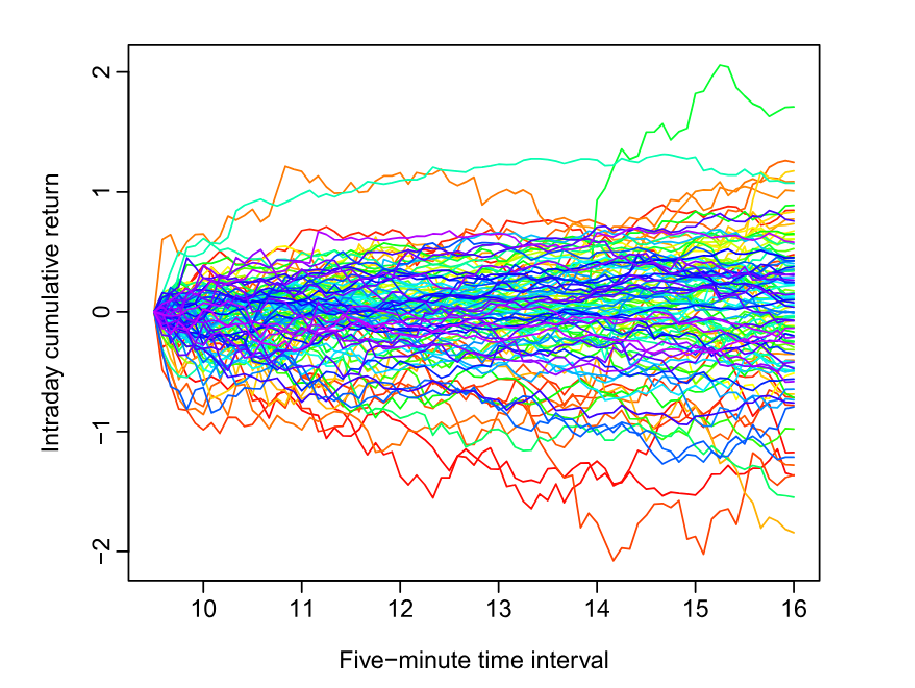
\includegraphics[width=0.98\linewidth,height=4.55cm,keepaspectratio]{intraday_cumulative_return.pdf}

      {\scriptsize Functional cumulative intraday returns: one curve per trading day.}

    \column{0.37\textwidth}
      \uncover<2->{%
      \begin{beamercolorbox}[rounded=true,sep=0.55em,wd=\linewidth]{block body}
        \centering
        \alert<2>{\Large\(X_t(u)\)}\\[0.20cm]
        \raggedright
        \alert<2>{\textbf{\(t\)}}: which day\\[0.14cm]
        \alert<2>{\textbf{\(u\)}}: position within that day\\[0.14cm]
        \alert<2>{\textbf{\(X_t(u)\)}}: the complete daily shape
      \end{beamercolorbox}}

      \vspace{0.28cm}
      \uncover<3->{\centering\small
        \alert<3>{\textbf{Other examples}}\\[0.10cm]
        Electricity-demand curves\\[0.06cm]
        Financial yield curves\\[0.06cm]
        Highway traffic-flow curves}
  \end{columns}
  \src{Example adapted from Shang (2017), \emph{Journal of Forecasting}.}
  \note{Start with the object. A functional time series is not a long vector at one date; it is a sequence in which each date contributes a whole curve. Here each trading day is one intraday cumulative-return curve. The same structure appears in demand, yield, and traffic data.}
\end{frame}

% 0:45
\begin{frame}{FARMA describes two ways the past enters today}
  \centering
  \small\color{MidGray}For a stationary functional time series, write the curve at time \(t\) as \(Y_t\).

  \vspace{0.16cm}
  \color{black}
  \begin{beamercolorbox}[rounded=true,sep=0.48em,wd=0.96\linewidth]{block body}
    \centering\large
    \(\displaystyle
      Y_t=
      \uncover<1->{\alert<1>{\underbrace{\sum_{i=1}^{p}\Phi_iY_{t-i}}_{\text{past curves}}}}
      +\eta_t
      \uncover<2->{+\alert<2>{\underbrace{\sum_{j=1}^{q}\Theta_j\eta_{t-j}}_{\text{past shocks}}}}
    \)
  \end{beamercolorbox}

  \vspace{0.36cm}
  \begin{columns}[t,onlytextwidth]
    \column{0.47\textwidth}
      \uncover<1->{\centering
        \alert<1>{\textbf{Functional autoregression (FAR)}}\\[0.12cm]
        \small Yesterday's curves directly shape today's curve.\\[0.16cm]
        \alert<1>{\(p\) = number of curve lags}}
    \column{0.47\textwidth}
      \uncover<2->{\centering
        \alert<2>{\textbf{Functional moving average (FMA)}}\\[0.12cm]
        \small Recent unobserved shocks continue to echo.\\[0.16cm]
        \alert<2>{\(q\) = number of shock lags}}
  \end{columns}

  \vspace{0.40cm}
  \uncover<3->{\talktakeaway{\(\Phi_i,\Theta_j:\cH\to\cH\) map an entire input curve to an entire output curve; \(\cH=L^2(\mathcal U)\).}}
  \note{FARMA is the functional analogue of scalar ARMA. The FAR part is direct feedback from observed curves. The FMA part carries forward unobserved shocks. The orders p and q count how many of each type we keep, while Phi and Theta transform whole curves rather than multiplying single numbers.}
\end{frame}

% 0:40
\begin{frame}{Long memory keeps old shocks alive}
  \centering
  \begin{columns}[t,onlytextwidth]
    \column{0.32\textwidth}
      \uncover<1->{\centering
        \alert<1>{\textbf{Short memory: \(d=0\)}}\\[0.08cm]
        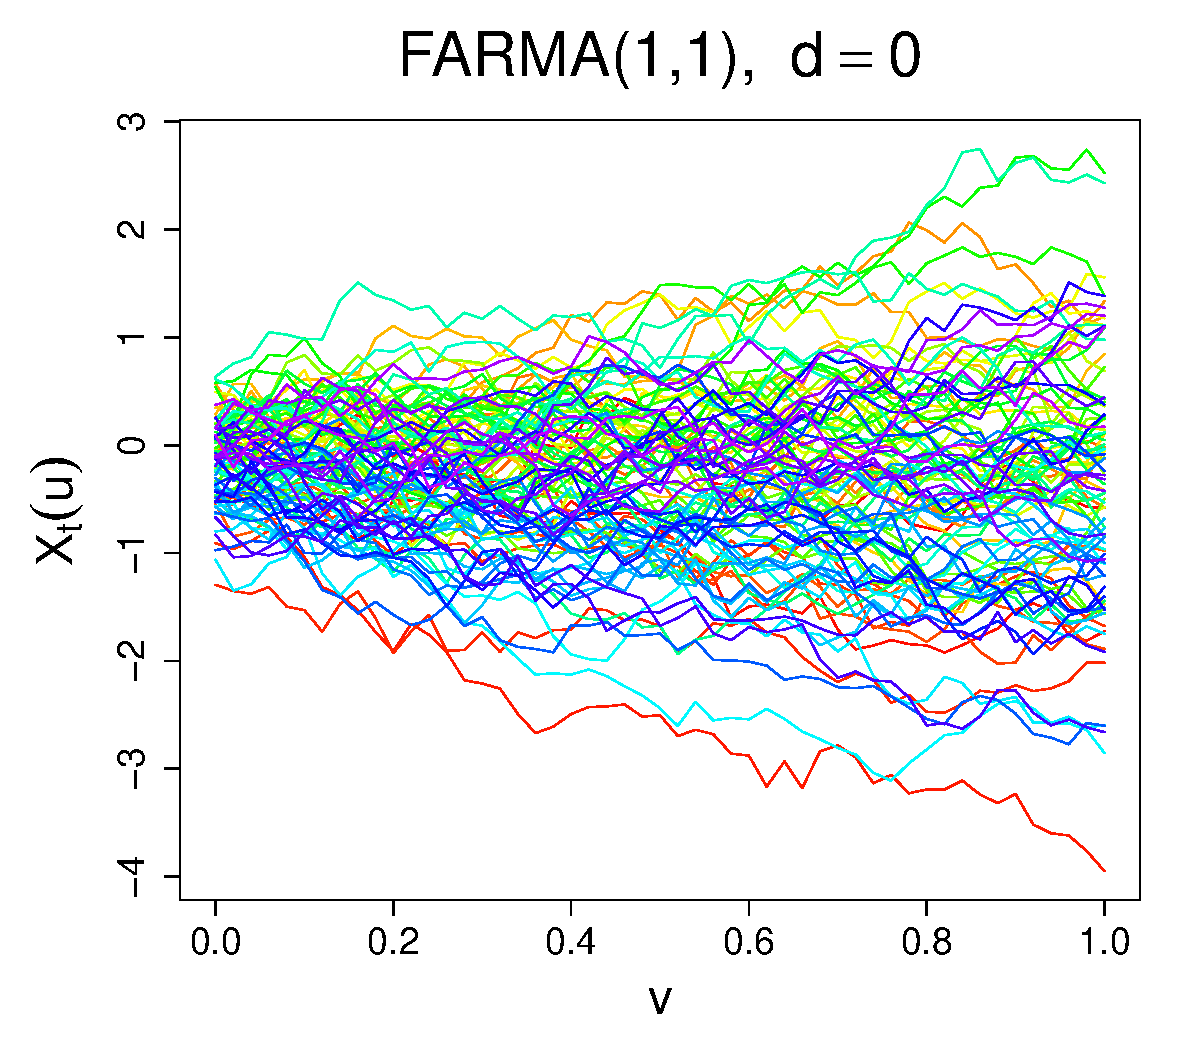
\includegraphics[width=3.55cm,height=3.05cm,keepaspectratio]{FARMA_0.pdf}}
    \column{0.32\textwidth}
      \uncover<2->{\centering
        \alert<2>{\textbf{Long memory: \(d=0.3\)}}\\[0.08cm]
        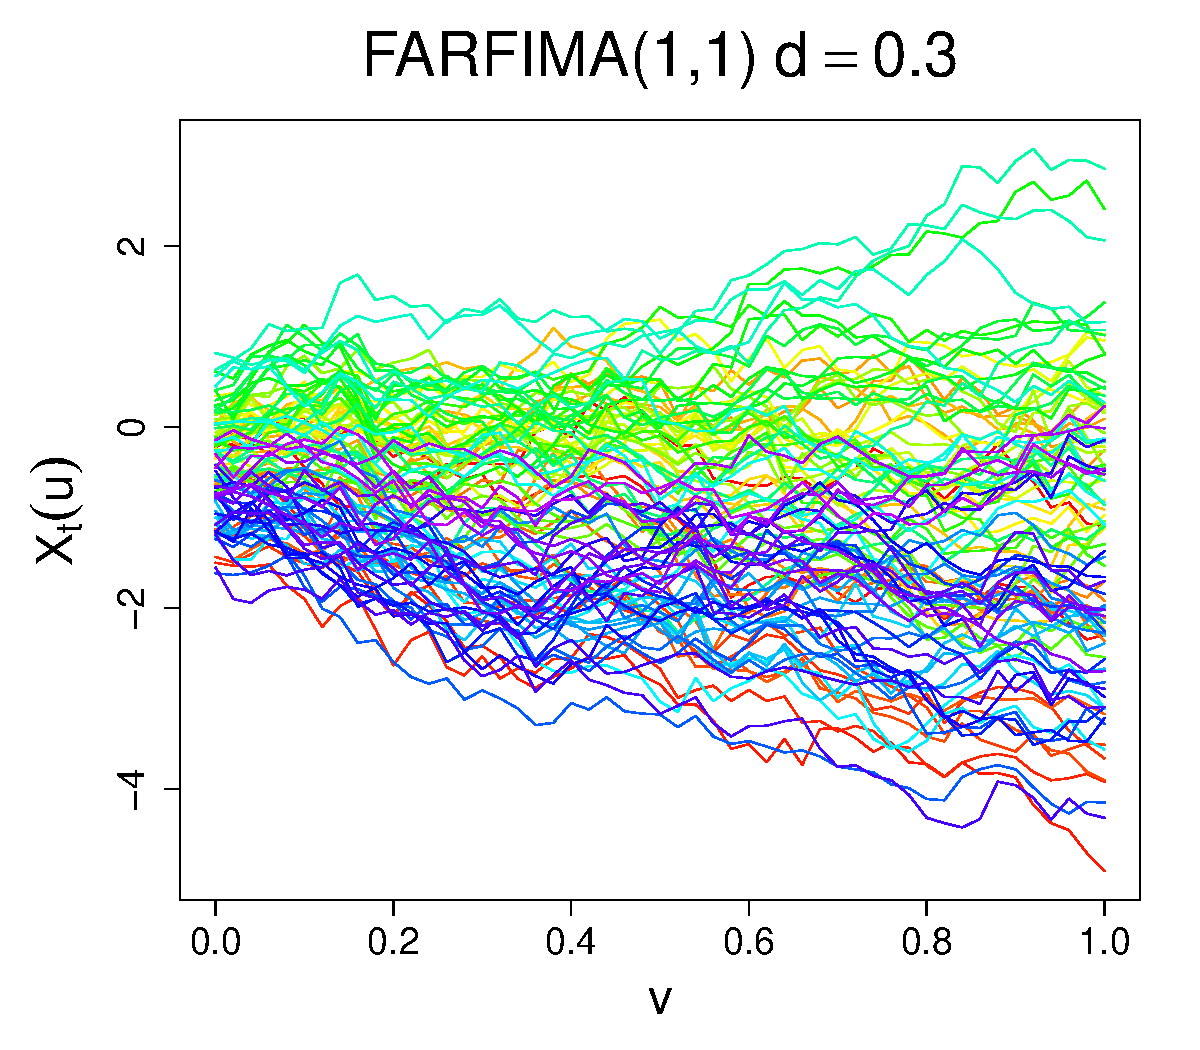
\includegraphics[width=3.55cm,height=3.05cm,keepaspectratio]{FARFIMA_03.pdf}}
    \column{0.32\textwidth}
      \uncover<3->{\centering
        \alert<3>{\textbf{Non-stationary: \(d=1\)}}\\[0.08cm]
        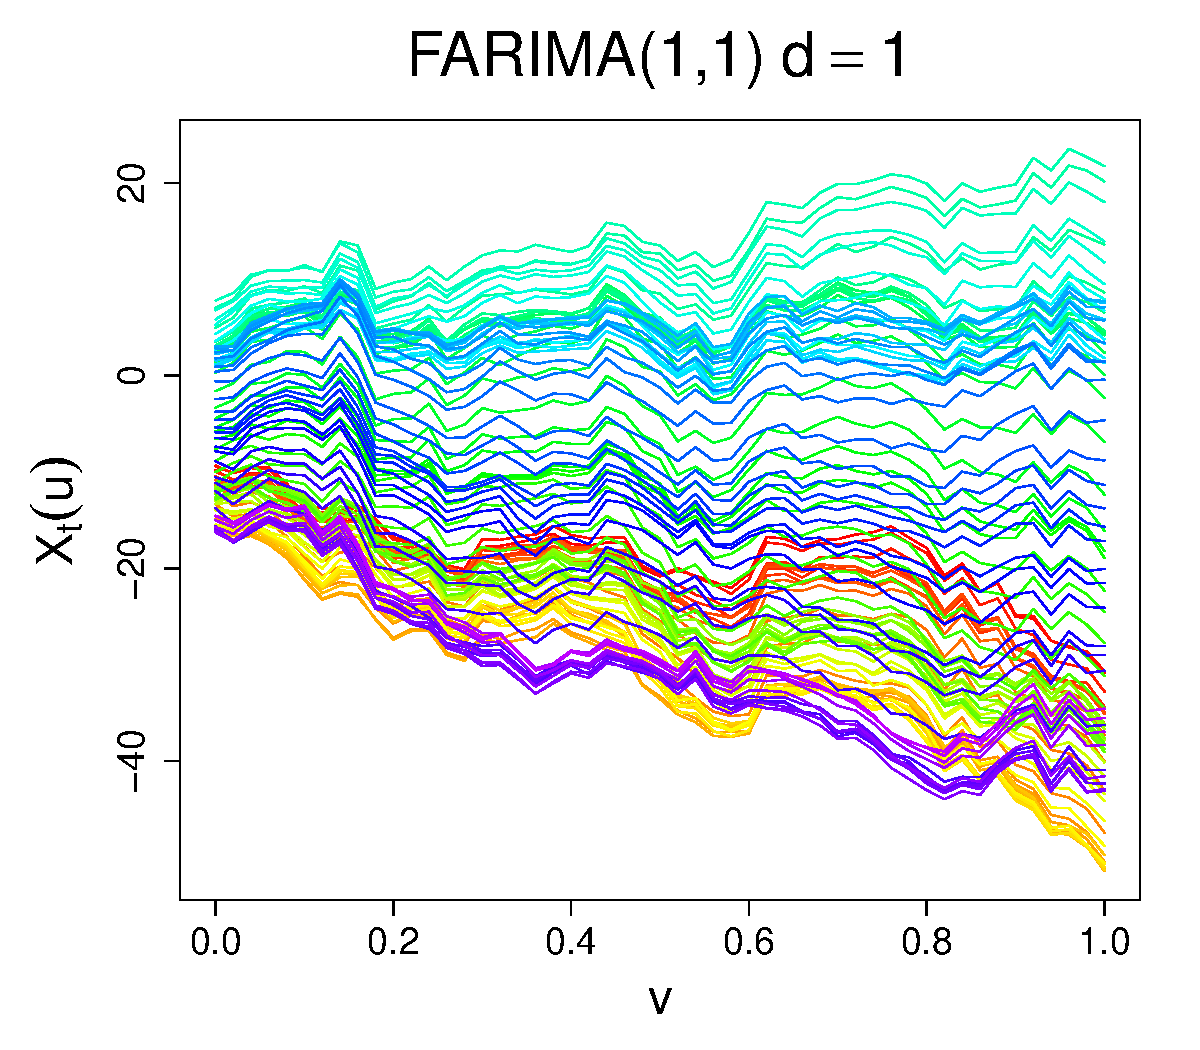
\includegraphics[width=3.55cm,height=3.05cm,keepaspectratio]{FARFIMA_1.pdf}}
  \end{columns}

  \vspace{0.24cm}
  \uncover<4->{\begin{beamercolorbox}[rounded=true,sep=0.35em,wd=0.94\linewidth]{block body}
    \centering\small
    \alert<4>{For \(0<d<\tfrac12\), dependence decays slowly; for \(d>\tfrac12\), variability can accumulate and the original process is non-stationary.}
  \end{beamercolorbox}}
  \note{The visual effect of d is persistence across curves. With d equal to zero, fluctuations are stable. With fractional d, old shocks fade very slowly. Beyond one half the original process is non-stationary, so its variability changes over time. The examples have identical physical dimensions to support direct comparison.}
\end{frame}

% 0:35
\begin{frame}{FARFIMA\((p,d,q)\) separates three sources of dependence}
  \centering
  \begin{tikzpicture}[x=1cm,y=1cm]
    \node[font=\Large\bfseries] at (-1.85,1.72) {FARFIMA};
    \node[font=\Large] at (-0.58,1.72) {\((\)};
    \node[font=\Large\bfseries] (p) at (-0.25,1.72) {\alert<1>{\(p\)}};
    \node[font=\Large] at (0.08,1.72) {,};
    \node[font=\Large\bfseries] (d) at (0.40,1.72) {\alert<2>{\(d\)}};
    \node[font=\Large] at (0.73,1.72) {,};
    \node[font=\Large\bfseries] (q) at (1.05,1.72) {\alert<3>{\(q\)}};
    \node[font=\Large] at (1.38,1.72) {\()\)};

    \uncover<1->{\node[panel,anchor=north] (ar) at (-3.70,1.03) {
      \begin{minipage}[t][1.34cm][t]{3.00cm}
        \centering\alert<1>{\panelheading{Autoregression}}\\[0.12cm]
        \alert<1>{\panelbody{\(p\): number of past-curve lags}}
      \end{minipage}};
      \draw[flowarrow] (p.south)--(ar.north);}
    \uncover<2->{\node[panelred,anchor=north] (memory) at (0,1.03) {
      \begin{minipage}[t][1.34cm][t]{3.00cm}
        \centering\alert<2>{\panelheading{Memory}}\\[0.12cm]
        \alert<2>{\panelbody{\(d\): persistence parameter}}
      \end{minipage}};
      \draw[flowarrow] (d.south)--(memory.north);}
    \uncover<3->{\node[panel,anchor=north] (ma) at (3.70,1.03) {
      \begin{minipage}[t][1.34cm][t]{3.00cm}
        \centering\alert<3>{\panelheading{Moving average}}\\[0.12cm]
        \alert<3>{\panelbody{\(q\): number of past-shock lags}}
      \end{minipage}};
      \draw[flowarrow] (q.south)--(ma.north);}

    \uncover<4->{
      \node[font=\large] at (0,-1.38) {
        \(Y_t\sim\operatorname{FARMA}(p,q)
          \xrightarrow{\ (1-B)^{-d}\ }
          X_t\sim\operatorname{FARFIMA}(p,d,q)\)};}

    \uncover<5->{\node[panel,anchor=north] at (-2.80,-2.02) {
      \begin{minipage}[t][0.78cm][c]{4.10cm}
        \centering\alert<5>{\panelheading{Selection problem}}
      \end{minipage}};
      \node[panelred,anchor=north] at (2.80,-2.02) {
      \begin{minipage}[t][0.78cm][c]{4.10cm}
        \centering\alert<5>{\panelheading{Forecasting problem}}
      \end{minipage}};}
  \end{tikzpicture}
  \note{The notation separates the three modelling tasks directly. The autoregressive order p counts curve lags, d controls long-run persistence, and the moving-average order q counts shock lags. Fractional integration maps a stationary FARMA process Y into the observed FARFIMA process X. The thesis addresses both the resulting selection problem and the forecasting problem.}
\end{frame}

\section{Literature \& gap}

% 0:55
\begin{frame}{The literature leaves the full workflow disconnected}
  \centering
  \renewcommand{\arraystretch}{1.23}
  \small
  \begin{tabularx}{0.97\linewidth}{>{\bfseries\raggedright\arraybackslash}p{2.55cm} >{\raggedright\arraybackslash}X >{\raggedright\arraybackslash}p{3.25cm}}
    \toprule
    Stream & What is established & The gap \\
    \midrule
    \uncover<1->{\alert<1>{Estimation of memory parameter}} &
      \uncover<1->{Dominant subspaces and estimation of \(d\)} &
      \\
    \uncover<2->{\alert<2>{Functional order selection}} &
      \uncover<2->{fACF/fPACF; sequential FAR tests} &
      \uncover<2->{Diagnostic or pure-FAR restrictions} \\
    \uncover<3->{\alert<3>{Functional forecasting}} &
      \uncover<3->{FARFIMA\((1,1,0)\)} &
      \uncover<3->{No fractional differencing; no moving-average term} \\
    \bottomrule
  \end{tabularx}

  \vspace{0.22cm}
  \uncover<4->{\begin{beamercolorbox}[rounded=true,sep=0.42em,wd=0.96\linewidth]{block body alerted}
    \centering\small\bfseries
    \alert<4>{Gap: estimate \(d\), select both \(p\) and \(q\), estimate the operators, and produce calibrated forecasts on the original functional scale in one theoretically grounded workflow.}
  \end{beamercolorbox}}
  \src{Li et al. (2020, 2023); Kokoszka and Reimherr (2013); Mestre et al. (2021); Klepsch et al. (2017).}
  \note{The literature provides strong ingredients, but mostly as separate streams. Long-memory work estimates the persistent subspace and d. Order-identification work supplies diagnostics, pure-FAR tests, or prediction-based selection. Forecasting work starts after specification. The gap is to connect structural order recovery with long-memory preprocessing and original-scale uncertainty.}
\end{frame}

\section{Methodology}

% 0:45
\begin{frame}{This thesis connects the pieces in one estimable workflow}
  \centering
  \begin{tikzpicture}[x=1cm,y=1cm]
    \uncover<1->{\node[panel,anchor=north] (mem) at (-3.70,0) {
      \begin{minipage}[t][3.55cm][t]{3.00cm}
        \centering\alert<1>{\panelheading{1. Memory}}\\[0.18cm]
        \small
        Compare covariance operators\\[0.13cm]
        Dominant score + BC--LPWN
        \vfill
        \alert<1>{Estimate \(d\) and difference}
      \end{minipage}};}
    \uncover<2->{\node[panelred,anchor=north] (dyn) at (0,0) {
      \begin{minipage}[t][3.55cm][t]{3.00cm}
        \centering\alert<2>{\panelheading{2. Dynamics}}\\[0.18cm]
        \small
        Functional Box--Jenkins\\[0.13cm]
        Adaptive functional HQ\\[0.13cm]
        Hannan--Rissanen estimation
        \vfill
        \alert<2>{Select \((p,q)\) and fit}
      \end{minipage}};}
    \uncover<3->{\node[panelgreen,anchor=north] (pred) at (3.70,0) {
      \begin{minipage}[t][3.55cm][t]{3.00cm}
        \centering\alert<3>{\panelheading{3. Prediction}}\\[0.18cm]
        \small
        Plug-in point forecasts\\[0.13cm]
        Fractional integration\\[0.13cm]
        Conformal calibration
        \vfill
        \alert<3>{Return to the original scale}
      \end{minipage}};}
    \uncover<2->{\draw[flowarrow] (mem)--(dyn);}
    \uncover<3->{\draw[flowarrow] (dyn)--(pred);}
  \end{tikzpicture}

  \vspace{0.40cm}
  \uncover<4->{\talktakeaway{The simulations first isolate each component, then evaluate the complete FARFIMA pipeline.}}
  \note{The contribution is a connected workflow. First estimate the memory and stationarise the curves. Then select and estimate the short-run dynamics. Finally forecast, reintegrate, and calibrate uncertainty on the scale users observe. The simulations follow the same logic: components first, then the unified pipeline.}
\end{frame}

% 0:50
\begin{frame}{Step 1: estimate \(d\) along the dominant memory direction}
  \centering
  \begin{tikzpicture}[x=1cm,y=1cm]
    \uncover<1->{\node[panel,anchor=north] (s) at (-3.70,1.20) {
      \begin{minipage}[t][1.62cm][t]{3.00cm}
        \centering\alert<1>{\panelheading{Sample covariance}}\\[0.16cm]
        \normalsize\alert<1>{\(\displaystyle \widehat V_T^{\mathrm{Covar}}
          =\sum_{t=1}^{T}X_t\otimes X_t\)}
      \end{minipage}};
    \node[panel,anchor=north] (rs) at (0,1.20) {
      \begin{minipage}[t][1.62cm][t]{3.00cm}
        \centering\alert<1>{\panelheading{Rescaled LRC}}\\[0.16cm]
        \normalsize\alert<1>{\(\displaystyle \widehat V_T^{\mathrm{RS}}
          =\sum_kW_q\!\left(\frac{k}{\widehat h}\right)\widehat r_k\)}
      \end{minipage}};
    \node[panel,anchor=north] (lrs) at (3.70,1.20) {
      \begin{minipage}[t][1.62cm][t]{3.00cm}
        \centering\alert<1>{\panelheading{Sandwich LRC}}\\[0.16cm]
        \normalsize\alert<1>{\(\displaystyle \widehat V_T^{\mathrm{LRS}}
          =\sum_{|k|\le m}(m-|k|)\widehat r_k\)}
      \end{minipage}};}

    \uncover<2->{
      \coordinate (sb) at ($(s.south)+(0,-0.18)$);
      \coordinate (rsb) at ($(rs.south)+(0,-0.18)$);
      \coordinate (lrsb) at ($(lrs.south)+(0,-0.18)$);
      \draw[CNU,line width=1.05pt] (s.south)--(sb);
      \draw[CNU,line width=1.05pt] (rs.south)--(rsb);
      \draw[CNU,line width=1.05pt] (lrs.south)--(lrsb);
      \draw[CNU,line width=1.05pt] (sb)--(lrsb);
      \node[panel,anchor=north] (fpca) at (0,-1.28) {
        \begin{minipage}[t][0.72cm][c]{4.10cm}
          \centering\alert<2>{\panelheading{1. FPCA direction}}\\[-0.01cm]
          \alert<2>{\panelbody{Extract the leading eigenfunction \(\widehat\psi_1\)}}
        \end{minipage}};
      \draw[flowarrow] (rsb)--(fpca.north);}

    \uncover<3->{\node[panel,anchor=north] (score) at (0,-2.55) {
      \begin{minipage}[t][0.72cm][c]{4.10cm}
        \centering\alert<3>{\panelheading{2. Score process}}\\[-0.01cm]
        \alert<3>{\panelbody{\(\widehat\xi_{t,1}=\langle X_t,\widehat\psi_1\rangle\)}}
      \end{minipage}};
      \draw[flowarrow] (fpca.south)--(score.north);}
    \uncover<4->{\node[panelred,anchor=north] (lpwn) at (0,-3.82) {
      \begin{minipage}[t][0.72cm][c]{4.10cm}
        \centering\alert<4>{\panelheading{3. Memory estimate}}\\[-0.01cm]
        \alert<4>{\panelbody{BC--LPWN estimates \(\widehat d_{\mathrm{BC}}\)}}
      \end{minipage}};
      \draw[flowarrow] (score.south)--(lpwn.north);}
  \end{tikzpicture}
  \note{Three covariance constructions are compared because dominant-subspace recovery comes before memory estimation. Their leading eigenfunction generates a scalar score. LPWN models low-frequency curvature around the power law, and the prefiltered sieve bootstrap corrects remaining finite-sample bias.}
\end{frame}

% 0:55
\begin{frame}{Step 2: residual dependence selects the FARMA order}
  \centering
  \uncover<1->{%
  \begin{beamercolorbox}[rounded=true,sep=0.34em,wd=0.96\linewidth]{block body}
    \centering
    \alert<1>{\(\displaystyle
      \widehat\Gamma_h^{(p,q)}
      =\frac1T\sum_{t=h+1}^{T}
      \widehat\eta_t^{(p,q)}\otimes\widehat\eta_{t-h}^{(p,q)}
    \)}\\[-0.02cm]
    \scriptsize \(\widehat\eta_t^{(p,q)}\): residual curve from the fitted FARMA\((p,q)\);
    \(\widehat\Gamma_h^{(p,q)}\): its lag-\(h\) empirical autocovariance operator; \(\|\cdot\|\): Hilbert--Schmidt norm.
  \end{beamercolorbox}}

  \vspace{0.10cm}
  \begin{tikzpicture}[x=1cm,y=1cm]
    \uncover<2->{\node[panel,anchor=north] (bj) at (-2.85,0) {
      \begin{minipage}[t][2.65cm][t]{4.70cm}
        \centering\alert<2>{\panelheading{Functional Box--Jenkins}}\\[0.12cm]
        \small Increase complexity; stop at the first residual-white-noise model.\\[0.13cm]
        \alert<2>{\resizebox{0.91\linewidth}{!}{\(\displaystyle
          V_{T,H}^{(p,q)}
          =T\sum_{h=1}^{H}\left\|\widehat\Gamma_h^{(p,q)}\right\|^2,
          \qquad H=\lfloor\log T\rfloor
        \)}}
      \end{minipage}};}
    \uncover<3->{\node[panelred,anchor=north] (hq) at (2.85,0) {
      \begin{minipage}[t][2.65cm][t]{4.70cm}
        \centering\alert<3>{\panelheading{Adaptive functional HQ}}\\[0.12cm]
        \small Compare all candidates; penalise unnecessary FARMA lags.\\[0.10cm]
        \alert<3>{\resizebox{0.79\linewidth}{!}{\(\displaystyle
          F_T(p,q)=\frac1H\sum_{h=1}^{H}
          \left\|\widehat\Gamma_h^{(p,q)}\right\|^2
        \)}}\\[0.04cm]
        \alert<3>{\resizebox{0.94\linewidth}{!}{\(\displaystyle
          \IC_T(p,q)=F_T(p,q)
          +\log\!\log(T)\,\widehat\delta_T(p+q)
        \)}}
      \end{minipage}};}
  \end{tikzpicture}
  \note{Both methods are built from residual autocovariance operators. Box--Jenkins is sequential and can stop early. The adaptive HQ criterion compares residual dependence globally with a data-scaled Hannan--Quinn penalty and is consistent over the finite candidate set.}
\end{frame}

% 0:35
\begin{frame}{Step 3: reconstruct hidden shocks before estimating the operators}
  \centering
  \uncover<1->{\large
    The moving-average shocks \alert<1>{\(\eta_t\)} are not observed.}

  \vspace{0.38cm}
  \begin{tikzpicture}[x=1cm,y=1cm]
    \uncover<2->{\node[panel,anchor=north] (proxy) at (-3.70,0) {
      \begin{minipage}[t][2.45cm][t]{3.00cm}
        \centering\alert<2>{\panelheading{1. Fit a flexible FAR proxy}}\\[0.22cm]
        \small Use many observed curve lags to approximate the full dependence.
      \end{minipage}};}
    \uncover<3->{\node[panelred,anchor=north] (shocks) at (0,0) {
      \begin{minipage}[t][2.45cm][t]{3.00cm}
        \centering\alert<3>{\panelheading{2. Recover proxy shocks}}\\[0.22cm]
        \small Treat the residual curves as estimates of the hidden innovations.
      \end{minipage}};
      \draw[flowarrow] (proxy)--(shocks);}
    \uncover<4->{\node[panelgreen,anchor=north] (joint) at (3.70,0) {
      \begin{minipage}[t][2.45cm][t]{3.00cm}
        \centering\alert<4>{\panelheading{3. Estimate}\\[-0.01cm]
          \panelheading{jointly}}\\[0.22cm]
        \small Regress on curve lags and proxy-shock lags to estimate \(\Phi_i\) and \(\Theta_j\).
      \end{minipage}};
      \draw[flowarrow] (shocks)--(joint);}
  \end{tikzpicture}

  \vspace{0.40cm}
  \uncover<5->{\talktakeaway{Hannan--Rissanen turns a hidden-shock problem into a functional regression.}}
  \note{The main idea is simple. First fit a rich functional autoregression. Its residual curves approximate the innovations we cannot observe. Then use both observed curve lags and recovered shock lags in one regression to estimate the FAR and FMA operators. The projected-operator formulas and regularised inverses are in backup.}
\end{frame}

% 0:45
\begin{frame}{Step 4: the proposed forecast estimates what the benchmark fixes}
  \centering
  \begin{tikzpicture}[node distance=0.30cm]
    \uncover<1->{\node[panel,text width=5.12cm,minimum height=3.75cm] (base) {
      \alert<1>{\panelheading{Benchmark: FARFIMA\((1,1,0)\)}}\\[0.18cm]
      \alert<1>{\(\displaystyle \Delta X_t=\Phi_1\Delta X_{t-1}+\eta_t.\)}\\[0.18cm]
      Fix \(d=1\), \(p=1\), \(q=0\): first-difference the curves and fit FAR\((1)\).
    };}
    \uncover<2->{\node[panelred,text width=5.12cm,minimum height=3.75cm,right=of base] (prop) {
      \alert<2>{\panelheading{Proposed plug-in forecast}}\\[0.18cm]
      Estimate \(d\), select \((p,q)\), and estimate every operator.\\[0.18cm]
      \alert<2>{\(\displaystyle \widehat X_{T+h|T}
          =(1-B)^{-\widehat d}\widehat Y_{T+h|T}.\)}
    };}
  \end{tikzpicture}

  \vspace{0.24cm}
  \uncover<3->{\alert<3>{\(\displaystyle
    \widehat Y_{T+h|T}
    =\sum_{i=1}^{p}\widehat\Phi_i\widehat Y_{T+h-i|T}
     +\sum_{j=1}^{q}\widehat\Theta_j\widehat\eta_{T+h-j|T},
    \qquad \widehat\eta_{s|T}=0\ \text{for }s>T.
  \)}}
  \note{The benchmark imposes both first differencing and a FAR one short-run structure. The proposed method can gain by estimating d, by selecting a better FARMA order, or both. Future innovations have conditional mean zero, so moving-average gains concentrate at short horizons.}
\end{frame}

% 0:50
\begin{frame}{Step 5: one validation set supports two tasks}
  \centering
  \begin{tikzpicture}[x=1cm,y=1cm]
    \uncover<1->{\node[panel,anchor=north] (train) at (-3.70,0) {
      \begin{minipage}[t][0.72cm][t]{3.00cm}
        \centering\alert<1>{\panelheading{Training}}\\[-0.02cm]
        \small Fit candidates
      \end{minipage}};
    \node[panelred,anchor=north] (val) at (0,0) {
      \begin{minipage}[t][0.72cm][t]{3.00cm}
        \centering\alert<1>{\panelheading{Validation}}\\[-0.02cm]
        \small Select + calibrate
      \end{minipage}};
    \node[panelgreen,anchor=north] (test) at (3.70,0) {
      \begin{minipage}[t][0.72cm][t]{3.00cm}
        \centering\alert<1>{\panelheading{Test}}\\[-0.02cm]
        \small Evaluate once
      \end{minipage}};}

    \uncover<2->{\node[panel,anchor=north] (cv) at (0,-1.35) {
      \begin{minipage}[t][1.55cm][t]{10.15cm}
        \alert<2>{\panelheading{1. Forecast CV chooses a predictive order}}\\[0.10cm]
        \small Average the \(h\)-step squared validation error on the original scale.\\[0.12cm]
        \centering\alert<2>{\(\displaystyle
          (\widehat p_{\rm CV},\widehat q_{\rm CV})
          =\arg\min_{(p,q)\in\cM}\mathrm{CV}_h(p,q)
        \)}
      \end{minipage}};}

    \uncover<3->{\node[panelred,anchor=north] (conf) at (0,-3.70) {
      \begin{minipage}[t][1.70cm][t]{10.15cm}
        \alert<3>{\panelheading{2. Conformal calibration chooses the band width}}\\[0.10cm]
        \small Choose the smallest residual multiplier reaching target coverage \(1-\alpha\).\\[0.10cm]
        \centering\alert<3>{\(\displaystyle
          \widehat\zeta_{\alpha,h}
          =\inf\{z:\ECP_h(z)\ge1-\alpha\},
          \qquad
          \widehat X_{T+h|T}(u)\pm
          \widehat\zeta_{\alpha,h}\gamma_h(u)
        \)}
      \end{minipage}};}
  \end{tikzpicture}
  \note{The validation set has two roles. Forecast cross-validation is a useful byproduct and predictive benchmark for choosing orders. Separately, residual curves calibrate one conformal multiplier per horizon after returning to the original scale. Window mechanics are illustrated in backup.}
\end{frame}

% 0:35
\begin{frame}{Evaluation I: structure recovery and point forecasting}
  \centering
  \begin{tikzpicture}[x=1cm,y=1cm]
    \node[panel,anchor=north] (ord) at (-2.85,0) {
      \begin{minipage}[t][3.45cm][t]{4.70cm}
        \centering\panelheading{Exact order recovery}\\[0.32cm]
        \(\displaystyle
          \mathrm{Accuracy}=\frac1R\sum_{r=1}^{R}
          \mathbf 1\!\left\{(\widehat p_r,\widehat q_r)=(p_0,q_0)\right\}
        \)\\[0.45cm]
        \metriccue{GoodGreen}{Higher is better}
      \end{minipage}};
    \node[panel,anchor=north] (rmse) at (2.85,0) {
      \begin{minipage}[t][3.45cm][t]{4.70cm}
        \centering\panelheading{Point forecasting}\\[0.22cm]
        \(\displaystyle
          \RMSE_h^{(a)}=
          \left\{\frac{1}{M_hN}\sum_{m,j}e_{m,h}^{(a)}(u_j)^2\right\}^{1/2}
        \)\\[0.08cm]
        {\small\(\displaystyle \mathrm{RMSE\ ratio}
          =\RMSE_h^{(a)}/\RMSE_h^{(1,1,0)}\)\\[0.04cm]
        }
        \metriccue{RevealRed}{Below one is better}
      \end{minipage}};
  \end{tikzpicture}

  \vspace{0.20cm}
  \begin{beamercolorbox}[rounded=true,sep=0.42em,wd=0.96\linewidth]{block body}
    \footnotesize
    \(R\): replications; \((p_0,q_0)\): true order; \((\widehat p_r,\widehat q_r)\): order selected in replication (r).\\[0.05cm]
    \(a\): method; \(h\): horizon; \(m=1,\ldots,M_h\): forecast origins; \(u_j, j=1,\ldots,N\): grid points;
    \(e_{m,h}^{(a)}(u_j)=X_{m+h}(u_j)-\widehat X_{m+h|m}^{(a)}(u_j)\).
  \end{beamercolorbox}
  \note{Structural recovery and predictive performance are separate questions. Exact order accuracy measures whether both p and q are correct. Point-forecast RMSE is reported relative to the FARFIMA one-one-zero benchmark.}
\end{frame}

% 0:35
\begin{frame}{Evaluation II: interval calibration and sharpness}
  \centering
  \begin{tikzpicture}[x=1cm,y=1cm]
    \node[panel,anchor=north] (ecp) at (-2.85,0) {
      \begin{minipage}[t][3.48cm][t]{4.70cm}
        \centering\panelheading{Empirical coverage probability}\\[0.30cm]
        \(\displaystyle
          \ECP_h=\frac{1}{M_hN}\sum_{m=1}^{M_h}\sum_{j=1}^{N}I_{m,h,j}
        \)\\[0.42cm]
        \metriccue{GoodGreen}{Target: \(1-\alpha\)}
      \end{minipage}};
    \node[panel,anchor=north] (score) at (2.85,0) {
      \begin{minipage}[t][3.48cm][t]{4.70cm}
        \centering\panelheading{Interval score: width + miss penalty}\\[0.12cm]
        {\small\(\displaystyle
          \mathrm{IS}_{\alpha}(X,L,U)
          =(U-L)+\frac{2}{\alpha}\bigl\{(L-X)_+ +(X-U)_+\bigr\}
        \)}\\[0.16cm]
        {\small\(\displaystyle \mathrm{Score\ ratio}
          =\frac{S_{\alpha,h}^{(a)}}{S_{\alpha,h}^{(1,1,0)}}\)}\\[0.08cm]
        \metriccue{RevealRed}{Below one is better}
      \end{minipage}};
  \end{tikzpicture}

  \vspace{0.18cm}
  \begin{beamercolorbox}[rounded=true,sep=0.42em,wd=0.96\linewidth]{block body}
    \footnotesize
    \(I_{m,h,j}=\mathbf1\{X_{m+h}(u_j)\in[L_{m,h,j},U_{m,h,j}]\}\).\\[0.05cm]
    \(L,U\): band limits; \(X\): realised value; \((x)_+=\max(x,0)\); \(\alpha\): miscoverage.\\[0.05cm]
    \(S_{\alpha,h}^{(a)}=(M_hN)^{-1}
      \sum_{m=1}^{M_h}\sum_{j=1}^{N}\mathrm{IS}_{\alpha,m,h,j}^{(a)}\):
    mean interval score across origins and grid points.\\[0.05cm]
    \(m,j,h,a,M_h,N\) are defined as on the preceding slide.
  \end{beamercolorbox}
  \note{Coverage alone rewards excessively wide intervals, so sharpness is evaluated with the interval score. The score combines width with penalties for observations below or above the band, and is again reported relative to the benchmark.}
\end{frame}

\section{Simulation}
\subsection{Component simulations}

% 0:30
\begin{frame}{Component 1: covariance operators and memory estimation}
  \centering
  \simplot{Cov_LW_FAR_tight.pdf}
  \note{This study isolates the dominant-subspace construction under FARFIMA one-d-zero, across sample sizes, memory parameters, and autoregressive strengths. The sample, rescaled long-run, and sandwich long-run operators give nearly identical memory estimates. Bias rises mainly when the short-run autoregressive operator is strong.}
\end{frame}

% 0:30
\begin{frame}{Component 2a: pure FAR and FMA order selection}
  \centering
  \simplot{order_accuracy_far_fma_2x2_tight.pdf}
  \note{This stationary study covers true orders one-zero, two-zero, zero-one, and zero-two over three sample sizes and strengths. Pure orders become easier with sample size and signal. Box--Jenkins can stop too early in weak FMA settings, while adaptive HQ is more stable.}
\end{frame}

% 0:30
\begin{frame}{Component 2b: mixed FARMA order selection}
  \centering
  \simplot{order_accuracy_farma_2x2_tight.pdf}
  \note{The mixed study covers true orders one-one, two-one, one-two, and two-two. Separating AR and MA effects is harder when both are present, because neighbouring FAR and FMA orders can generate similar residual dependence.}
\end{frame}

% 0:30
\begin{frame}{Component 3a: ideal point forecasting with true \(d\) and \((p,q)\)}
  \centering
  \simplot{forecast_rmse_ratio_2x2_tight.pdf}
  \note{This ideal study supplies the true d and true order and compares horizons one through ten under expanding and fixed windows. It isolates the value of the correct short-run structure. The benchmark is matched only for FARFIMA one-one-zero, and MA gains concentrate at short horizons.}
\end{frame}

% 0:30
\begin{frame}{Component 3b: ideal conformal coverage}
  \centering
  \simplot{forecast_ecp_95_expanding_2x2_tight.pdf}
  \note{These are 95 percent split-conformal bands on the original functional scale for horizons one through ten. Coverage remains close to nominal. The separate interval-score analysis in backup evaluates whether this calibration is achieved sharply.}
\end{frame}

\subsection{Unified simulation}

% 0:35
\begin{frame}{Unified 1: order selection after estimating \(d\)}
  \centering
  \simplot{unified_order_accuracy_T1000_2x2_tight.pdf}
  \note{Now every earlier stage is estimated for T equal to one thousand across d values and four true orders. Error in d propagates into the stationary transformation. Even so, adaptive functional HQ substantially outperforms forecast-based cross-validation for structural recovery.}
\end{frame}

% 0:35
\begin{frame}{Unified 2: point forecasting after estimating memory and order}
  \centering
  \simplot{unified_rmse_ratio_balanced_expanding_T1000_2x2_tight.pdf}
  \note{This is the end-to-end expanding-window result. The framework improves over the benchmark through two channels: correct fractional reconstruction when d differs from one, and richer selected short-run dynamics when truth is not FAR one.}
\end{frame}

\section{Conclusion}

% 0:45
\begin{frame}{A complete route from persistent curves to calibrated forecasts}
  \centering
  \begin{tikzpicture}
    \node[draw=CNU,line width=1.1pt,rounded corners=2pt,fill=CNUWash,
      minimum width=11.25cm,minimum height=3.05cm] (outer) {};
    \draw[CNU,line width=0.8pt] ($(outer.north west)!0.333!(outer.north east)$)--($(outer.south west)!0.333!(outer.south east)$);
    \draw[CNU,line width=0.8pt] ($(outer.north west)!0.666!(outer.north east)$)--($(outer.south west)!0.666!(outer.south east)$);
    \uncover<1->{\node[align=center,text width=3.35cm,anchor=north]
      at ($(outer.north west)!0.166!(outer.north east)+(0,-0.15cm)$) {
      \alert<1>{\Large\bfseries 1. Separate}\\[0.20cm]
      {\normalfont\small Estimate \(d\) from the\\leading score; then\\difference the curves.}};}
    \uncover<2->{\node[align=center,text width=3.35cm,anchor=north]
      at ($(outer.north west)!0.500!(outer.north east)+(0,-0.15cm)$) {
      \alert<2>{\Large\bfseries 2. Select}\\[0.20cm]
      {\normalfont\small Use residual dependence\\to select \((p,q)\); adaptive\\HQ performs best overall.}};}
    \uncover<3->{\node[align=center,text width=3.35cm,anchor=north]
      at ($(outer.north west)!0.833!(outer.north east)+(0,-0.15cm)$) {
      \alert<3>{\Large\bfseries 3. Forecast}\\[0.20cm]
      {\normalfont\small Estimate FARMA effects,\\integrate back, and calibrate\\\mbox{conformal bands.}}};}
  \end{tikzpicture}

  \vspace{0.48cm}
  \uncover<4->{\large\alert<4>{\bfseries
  Estimate \(d\) \(\longrightarrow\) select \((p,q)\) with adaptive HQ
  \(\longrightarrow\) forecast and calibrate.}}

  \vspace{0.46cm}
  \uncover<5->{\large\color{CNU}\bfseries Questions}
  \note{The contribution is the coherent sequence. Each component is evaluated separately, then the full pipeline is tested. The main recommendation is to estimate d, use adaptive functional HQ for structural selection, then forecast and calibrate after fractional integration.}
\end{frame}

\appendix
\section{Backup}

\begin{frame}{Backup: expanding versus fixed rolling windows}
  \centering
  \begin{tikzpicture}[x=0.72cm,y=1cm]
    \node[anchor=east,font=\bfseries] at (-0.15,1.25) {Expanding};
    \foreach \x in {0,...,9} {
      \draw[fill=CNUWash,draw=CNU] (\x,0.90) rectangle ++(0.74,0.62);
    }
    \draw[fill=RevealRed!12,draw=RevealRed,line width=1pt] (9.0,0.90) rectangle ++(0.74,0.62);
    \draw[decorate,decoration={brace,mirror,amplitude=4pt},CNU] (0,0.80)--(8.74,0.80)
      node[midway,below=5pt,align=center]{\scriptsize all observations available at this origin};
    \node[anchor=west,align=left] at (10.05,1.20) {\scriptsize window grows\\[-1pt]\scriptsize lower variance};

    \node[anchor=east,font=\bfseries] at (-0.15,-0.55) {Fixed rolling};
    \foreach \x in {0,...,3} {
      \draw[fill=SoftGray,draw=MidGray!55] (\x,-0.90) rectangle ++(0.74,0.62);
    }
    \foreach \x in {4,...,8} {
      \draw[fill=CNUWash,draw=CNU] (\x,-0.90) rectangle ++(0.74,0.62);
    }
    \draw[fill=RevealRed!12,draw=RevealRed,line width=1pt] (9.0,-0.90) rectangle ++(0.74,0.62);
    \draw[decorate,decoration={brace,mirror,amplitude=4pt},CNU] (4,-1.00)--(8.74,-1.00)
      node[midway,below=5pt,align=center]{\scriptsize last \(L\) curves only};
    \node[anchor=west,align=left] at (10.05,-0.60) {\scriptsize old curve exits\\[-1pt]\scriptsize adapts to change};
  \end{tikzpicture}

  \vspace{0.55cm}
  \begin{columns}[c,onlytextwidth]
    \column{0.48\textwidth}
      \centering\small Expanding windows ask: \emph{does using all available history stabilise estimation?}
    \column{0.48\textwidth}
      \centering\small Fixed windows ask: \emph{can a recent-history fit adapt when the process changes?}
  \end{columns}

  \vspace{0.28cm}
  \scriptsize\color{MidGray}At every forecast origin, the next \(h\) curves remain out of sample; the same rule is repeated through validation and test.
\end{frame}

\begin{frame}{Backup: forecast cross-validation is a predictive order selector}
  \centering
  \begin{beamercolorbox}[rounded=true,sep=0.70em,wd=0.94\linewidth]{block body}
  \[
    \mathrm{CV}_h(p,q)
      =\frac{1}{|\mathcal V_h|N}
       \sum_{m\in\mathcal V_h}\sum_{j=1}^{N}
       \bigl\{X_{m+h}(u_j)-\widehat X_{m+h|m}^{(p,q)}(u_j)\bigr\}^2,
  \]
  \[
    (\widehat p_{\rm CV},\widehat q_{\rm CV})
      =\arg\min_{(p,q)\in\cM}\mathrm{CV}_h(p,q).
  \]
  \end{beamercolorbox}

  \vspace{0.30cm}
  \begin{tikzpicture}[node distance=0.34cm]
    \node[panel,text width=4.95cm,minimum height=2.05cm] (hq) {
      \textbf{Adaptive HQ asks a structural question}\\[0.12cm]
      Which order leaves the most\\nearly white residuals after\\penalising complexity?};
    \node[panelred,text width=4.95cm,minimum height=2.05cm,right=of hq] (cv) {
      \textbf{CV asks a predictive question}\\[0.12cm]
      Which order forecasts the held-out validation curves most accurately?};
  \end{tikzpicture}

  \vspace{0.18cm}
  \small CV is therefore a useful byproduct and benchmark, but it need not recover the data-generating order.
\end{frame}

\begin{frame}{Backup: functional Box--Jenkins white-noise hypotheses}
  \centering
  \uncover<1->{%
  \begin{beamercolorbox}[rounded=true,sep=0.48em,wd=0.94\linewidth]{block body}
    \centering
    \alert<1>{\(\displaystyle
      \Gamma_h^{(p,q)}
      =\mathbb E\!\left[
        \eta_t^{(p,q)}\otimes\eta_{t-h}^{(p,q)}
      \right],
      \qquad h\ge1
    \)}\\[0.05cm]
    \scriptsize Population lag-\(h\) autocovariance operator of the residual process from candidate \((p,q)\).
  \end{beamercolorbox}}

  \vspace{0.24cm}
  \uncover<2->{%
  \begin{columns}[c,onlytextwidth]
    \column{0.47\textwidth}
      \begin{beamercolorbox}[rounded=true,sep=0.62em,wd=\linewidth]{block body}
        \centering\alert<2>{\textbf{Null: residual white noise}}\\[0.18cm]
        \alert<2>{\(\displaystyle
          H_0:\ \Gamma_h^{(p,q)}=0,
          \quad h=1,\ldots,H
        \)}
      \end{beamercolorbox}
    \column{0.47\textwidth}
      \begin{beamercolorbox}[rounded=true,sep=0.62em,wd=\linewidth]{block body}
        \centering\alert<2>{\textbf{Alternative: dependence remains}}\\[0.18cm]
        \alert<2>{\(\displaystyle
          H_1:\ \Gamma_h^{(p,q)}\ne0
          \text{ for some }h\le H
        \)}
      \end{beamercolorbox}
  \end{columns}}

  \vspace{0.25cm}
  \uncover<3->{%
  \begin{beamercolorbox}[rounded=true,sep=0.48em,wd=0.94\linewidth]{block body}
    \centering
    \alert<3>{\(\displaystyle
      V_{T,H}^{(p,q)}
      =T\sum_{h=1}^{H}\|\widehat\Gamma_h^{(p,q)}\|^2
      \ \Rightarrow\ 
      \sum_{\ell=1}^{\infty}\xi_{\ell,H}Z_\ell^2
      \ \approx\ c\chi_\kappa^2
    \)}\\[0.06cm]
    \scriptsize
    \(c=\sigma_{V,H}^2/(2\mu_{V,H})\),
    \(\kappa=2\mu_{V,H}^2/\sigma_{V,H}^2\).
    Reject for a large statistic; the first candidate not rejected is selected.
  \end{beamercolorbox}}
\end{frame}

\begin{frame}{Backup: full grid search finds the global IC minimum}
  \centering
  \begin{beamercolorbox}[rounded=true,sep=0.45em,wd=0.88\linewidth]{block body}
    \centering
    \(\displaystyle
      \cM=\{0,\ldots,5\}^{2}\setminus\{(0,0)\}
    \)
  \end{beamercolorbox}

  \vspace{0.28cm}
  \begin{tikzpicture}[x=1cm,y=1cm]
    \node[panel,anchor=north] (fit) at (-3.70,0) {
      \begin{minipage}[t][1.88cm][t]{3.00cm}
        \centering\textbf{1. Fit every candidate}\\[0.12cm]
        \small Estimate the FARMA model for each \((p,q)\in\cM\).
      \end{minipage}};
    \node[panel,anchor=north] (score) at (0,0) {
      \begin{minipage}[t][1.88cm][t]{3.00cm}
        \centering\textbf{2. Compute every IC}\\[0.12cm]
        \small Retain candidates with finite \(\IC_T(p,q)\).
      \end{minipage}};
    \node[panelred,anchor=north] (choose) at (3.70,0) {
      \begin{minipage}[t][1.88cm][t]{3.00cm}
        \centering\textbf{3. Choose the minimum}\\[0.12cm]
        \small Compare all retained candidates once.
      \end{minipage}};
    \draw[flowarrow] (fit.east)--(score.west);
    \draw[flowarrow] (score.east)--(choose.west);
  \end{tikzpicture}

  \vspace{0.30cm}
  \begin{beamercolorbox}[rounded=true,sep=0.55em,wd=0.88\linewidth]{block body alerted}
    \centering\large
    \(\displaystyle
      (\widehat p,\widehat q)
      =\arg\min_{(p,q)\in\cM:\,\IC_T(p,q)<\infty}\IC_T(p,q)
    \)
  \end{beamercolorbox}

  \vspace{0.28cm}
  \small\color{CNU}\bfseries Guaranteed global minimum over \(\cM\), at the cost of fitting the full grid.
\end{frame}

\begin{frame}{Backup: automatic search follows improving neighbouring orders}
  \centering
  \begin{tikzpicture}[x=1cm,y=1cm]
    \node[panel,anchor=north] (scale) at (-2.85,0) {
      \begin{minipage}[t][1.52cm][t]{4.70cm}
        \centering\textbf{1. Estimate the penalty scale}\\[0.12cm]
        \small Fit the largest candidate and set
        \(\widehat\delta_T=F_T(5,5)\).
      \end{minipage}};
    \node[panel,anchor=north] (start) at (2.85,0) {
      \begin{minipage}[t][1.52cm][t]{4.70cm}
        \centering\textbf{2. Select the best starting model}\\[0.12cm]
        \small Compare \(\mathcal S=\{(2,2),(1,0),(0,1)\}\).
      \end{minipage}};
    \node[panel,anchor=north] (move) at (-2.85,-2.35) {
      \begin{minipage}[t][2.02cm][t]{4.70cm}
        \centering\textbf{3. Search the eight neighbours}\\[0.12cm]
        \small Try every valid \((p+\Delta p,q+\Delta q)\), where
        \((\Delta p,\Delta q)\in\{-1,0,1\}^{2}\setminus\{(0,0)\}\).
      \end{minipage}};
    \node[panelred,anchor=north] (stop) at (2.85,-2.35) {
      \begin{minipage}[t][2.02cm][t]{4.70cm}
        \centering\textbf{4. Move only when IC decreases}\\[0.12cm]
        \small Continue from the best improving neighbour; stop when none improves the current IC.
      \end{minipage}};
  \end{tikzpicture}

  \vspace{0.28cm}
  \small\color{CNU}\bfseries Lower computational cost; the returned order is a local, not necessarily global, IC minimum.
\end{frame}

\begin{frame}{Backup: functional IC consistency---criterion and stochastic scale}
  \centering
  \uncover<1->{%
  \begin{beamercolorbox}[rounded=true,sep=0.50em,wd=0.96\linewidth]{block body}
    \centering
    \alert<1>{\(\displaystyle
      \IC_T(p,q)=F_T(p,q)+\log\!\log(T)\,\widehat\delta_T(p+q),
      \qquad
      F_T(p,q)=\frac1H\sum_{h=1}^{H}\|\widehat\Gamma_h^{(p,q)}\|^2
    \)}
  \end{beamercolorbox}}

  \vspace{0.24cm}
  \uncover<2->{%
  \begin{beamercolorbox}[rounded=true,sep=0.48em,wd=0.96\linewidth]{block body}
    \centering
    \alert<2>{\(\displaystyle
      \delta_T(p,q)=\frac1H\sum_{h=1}^{H}
      \|\widehat\Gamma_h^{(p,q)}-\Gamma_h^{(p,q)}\|^2,
      \qquad
      \widehat\delta_T=\min_{(p,q)\in\cM}F_T(p,q)
    \)}
  \end{beamercolorbox}}

  \vspace{0.24cm}
  \uncover<3->{%
  \begin{beamercolorbox}[rounded=true,sep=0.52em,wd=0.96\linewidth]{block body}
    \centering
    Under the draft's uniform projected-operator rate conditions,
    \alert<3>{\(\displaystyle
      \widehat\Gamma_h-\Gamma_h
      =O_p(T^{-1/2})+O_p(r_T),
      \quad r_T=O_p(T^{-\eta})
    \)}\\[0.12cm]
    hence
    \alert<3>{\(\displaystyle
      \delta_T=O_p(T^{-1}+T^{-2\eta}),
      \qquad \log\!\log(T)\,\widehat\delta_T=o_p(1).
    \)}
  \end{beamercolorbox}}

  \vspace{0.18cm}
  \uncover<4->{\small\alert<4>{\bfseries Claim: for a finite candidate set with identifiable minimal true order \((p_0,q_0)\),
  \(\Pr\{(\widehat p,\widehat q)=(p_0,q_0)\}\to1\).}}
\end{frame}

\begin{frame}{Backup: functional IC consistency---underfitting}
  \centering
  \uncover<1->{%
  \begin{beamercolorbox}[rounded=true,sep=0.58em,wd=0.94\linewidth]{block body}
    \centering
    If \((p,q)\) underfits, at least one population residual autocovariance is non-zero. Therefore
    \alert<1>{\(\displaystyle
      F_T(p,q)-F_T(p_0,q_0)
      \xrightarrow{p}
      c_{p,q}
      :=\frac1H\sum_{h=1}^{H}\|\Gamma_h^{(p,q)}\|^2>0.
    \)}
  \end{beamercolorbox}}

  \vspace{0.34cm}
  \uncover<2->{%
  \begin{beamercolorbox}[rounded=true,sep=0.62em,wd=0.94\linewidth]{block body}
    \centering
    The adaptive penalty vanishes on the absolute scale:
    \alert<2>{\(\displaystyle
      \log\!\log(T)\,\widehat\delta_T
      \bigl[(p+q)-(p_0+q_0)\bigr]=o_p(1).
    \)}
  \end{beamercolorbox}}

  \vspace{0.34cm}
  \uncover<3->{%
    \alert<3>{\(\displaystyle
      \IC_T(p,q)-\IC_T(p_0,q_0)
      =c_{p,q}+o_p(1)>0
    \)}

    \vspace{0.20cm}
    \small Hence every underfitted candidate is rejected with probability tending to one.}
\end{frame}

\begin{frame}{Backup: functional IC consistency---overfitting and conclusion}
  \centering
  \uncover<1->{%
  \begin{beamercolorbox}[rounded=true,sep=0.56em,wd=0.94\linewidth]{block body}
    \centering
    For an overfitted candidate, both population residual autocovariances vanish, so
    \alert<1>{\(\displaystyle
      F_T(p,q)-F_T(p_0,q_0)=O_p(\delta_T).
    \)}
  \end{beamercolorbox}}

  \vspace{0.28cm}
  \uncover<2->{%
  \begin{beamercolorbox}[rounded=true,sep=0.52em,wd=0.94\linewidth]{block body}
    \centering
    Let \(\Delta k=(p+q)-(p_0+q_0)>0\). If
    \(\widehat\delta_T\asymp_p\delta_T\), then
    \alert<2>{\(\displaystyle
      \frac{\IC_T(p,q)-\IC_T(p_0,q_0)}{\delta_T}
      =O_p(1)+\log\!\log(T)
        \frac{\widehat\delta_T}{\delta_T}\,\Delta k
      \xrightarrow{p}+\infty.
    \)}
  \end{beamercolorbox}}

  \vspace{0.28cm}
  \uncover<3->{%
    \alert<3>{\(\displaystyle
      \Pr\!\left\{\IC_T(p,q)>\IC_T(p_0,q_0)\right\}\to1.
    \)}

    \vspace{0.18cm}
    \small A finite union over all wrong candidates combines this result with the underfitting argument and proves exact-order consistency.}

  \vspace{0.16cm}
  \scriptsize\color{MidGray}The proof uses the finite candidate set, identifiability, uniform covariance-estimation rates, and penalty-scale equivalence stated in the thesis draft.
\end{frame}

\begin{frame}{Backup: functional Hannan--Rissanen algorithm---recover proxy shocks}
  \centering
  \begin{tikzpicture}[x=1cm,y=1cm]
    \node[panel,anchor=north] (a) at (-4.10,0) {
      \begin{minipage}[t][1.66cm][t]{2.12cm}
        \centering\textbf{1. Choose \(m\)}\\[0.08cm]
        \small Fit a high-order FAR\((m)\), \(m>p+q\).
      \end{minipage}};
    \node[panel,anchor=north] (b) at (-1.38,0) {
      \begin{minipage}[t][1.66cm][t]{2.12cm}
        \centering\textbf{2. Form lags}\\[0.08cm]
        \small Stack the last \(m\) curves in \(Y_t^{(m)}\).
      \end{minipage}};
    \node[panel,anchor=north] (c) at (1.38,0) {
      \begin{minipage}[t][1.66cm][t]{2.12cm}
        \centering\textbf{3. Project}\\[0.08cm]
        \small Retain empirical eigenspaces.
      \end{minipage}};
    \node[panel,anchor=north] (d) at (4.10,0) {
      \begin{minipage}[t][1.66cm][t]{2.12cm}
        \centering\textbf{4. Regress}\\[0.08cm]
        \(\widehat A_m=\widehat\Delta_m\widehat\Gamma_m^\dagger\)
      \end{minipage}};
    \draw[flowarrow] (a)--(b);
    \draw[flowarrow] (b)--(c);
    \draw[flowarrow] (c)--(d);
  \end{tikzpicture}

  \vspace{0.28cm}
  \begin{beamercolorbox}[rounded=true,sep=0.40em,wd=0.92\linewidth]{block body}
  \begin{align*}
    \widehat\Gamma_m
      &=\frac{1}{T-m}\sum_{t=m+1}^{T}Y_t^{(m)}\otimes Y_t^{(m)},\\
    \widehat\Delta_m
      &=\frac{1}{T-m}\sum_{t=m+1}^{T}Y_t\otimes Y_t^{(m)},\\
    \widehat Z_{t,m}
      &=Y_t-\widehat A_mY_t^{(m)}.
  \end{align*}
  \end{beamercolorbox}

  \vspace{0.06cm}
  \parbox{0.88\linewidth}{\centering\scriptsize\color{CNU}\bfseries
    The residual curves \(\widehat Z_{t,m}\) are proxies\\
    for the unobserved innovations \(\eta_t\).}
\end{frame}

\begin{frame}{Backup: Hannan--Rissanen pass 2---joint operator estimates}
  \centering
  \begin{beamercolorbox}[rounded=true,sep=0.65em,wd=0.95\linewidth]{block body}
  \begin{align*}
    \widehat{\bm Y}_{t,m}
      &=\bigl(Y_{t-1},\ldots,Y_{t-p},
          \widehat Z_{t-1,m},\ldots,\widehat Z_{t-q,m}\bigr)^\top,\\
    \widehat\Gamma_{p,q}
      &=\frac1{T-m}\sum_t\widehat{\bm Y}_{t,m}
          \otimes\widehat{\bm Y}_{t,m},\\
    \widehat\Delta_{p,q}
      &=\frac1{T-m}\sum_tY_t\otimes\widehat{\bm Y}_{t,m},\\
    \bigl(\widehat\Phi_1,\ldots,\widehat\Phi_p,
      \widehat\Theta_1,\ldots,\widehat\Theta_q\bigr)
      &=\widehat\Delta_{p,q}\widehat\Gamma_{p,q}^{\dagger}.
  \end{align*}
  \end{beamercolorbox}

  \vspace{0.30cm}
  \begin{tikzpicture}[x=1cm,y=1cm]
    \node[panel,anchor=north] (p) at (-3.55,0) {
      \begin{minipage}[t][1.50cm][t]{2.82cm}
        \centering\textbf{Projection}\\[0.08cm]
        \small Makes the infinite-dimensional problem finite
      \end{minipage}};
    \node[panel,anchor=north] (g) at (0,0) {
      \begin{minipage}[t][1.50cm][t]{2.82cm}
        \centering\textbf{Generalised inverse}\\[0.08cm]
        \small Regularises weak directions
      \end{minipage}};
    \node[panelred,anchor=north] (j) at (3.55,0) {
      \begin{minipage}[t][1.50cm][t]{2.82cm}
        \centering\textbf{Joint regression}\\[0.08cm]
        \small Separates feedback from shock propagation
      \end{minipage}};
  \end{tikzpicture}
\end{frame}

\begin{frame}{Backup: DFA gives the same covariance-operator conclusion}
  \centering
  \simplot{Cov_DFA_FAR_tight.pdf}
\end{frame}

\begin{frame}{Backup: ideal 95\% interval-score ratios}
  \centering
  \simplot{forecast_score_ratio_95_2x2_tight.pdf}
\end{frame}

\begin{frame}{Backup: unified memory estimation}
  \centering
  \simplot{unified_d_estimation_T1000_tight.pdf}
\end{frame}

\begin{frame}{Backup: unified 95\% conformal coverage}
  \centering
  \simplot{unified_ecp_95_expanding_2x2_tight.pdf}
\end{frame}

\begin{frame}{Backup: unified 95\% interval-score ratios}
  \centering
  \simplot{unified_score_ratio_95_expanding_2x2_tight.pdf}
\end{frame}

\begin{frame}{Backup: simulation architecture}
  \centering
  \begin{tikzpicture}[node distance=0.34cm]
    \node[panel,text width=5.05cm,minimum height=3.90cm] (components) {
      \textbf{Component studies isolate\\one question at a time}\\[0.22cm]
      1. covariance operator\\+ memory estimator\\[0.15cm]
      2. order selection on\\stationary FARMA\\[0.15cm]
      3. point and interval forecasts\\with true \(d,(p,q)\)
    };
    \node[panelred,text width=5.05cm,minimum height=3.90cm,right=of components] (unified) {
      \textbf{Unified study estimates the entire pipeline}\\[0.22cm]
      Estimate \(d\) \(\to\) transform \(\to\) select \((p,q)\) \(\to\) estimate operators \(\to\) forecast \(\to\) integrate \(\to\) calibrate
    };
  \end{tikzpicture}

  \vspace{0.30cm}
  \small
  \begin{tabular}{c@{\qquad}c@{\qquad}c}
    100 replications & horizons \(h=1,\ldots,10\) & expanding and fixed windows
  \end{tabular}
\end{frame}

\end{document}
